\section{Experiments}
\label{sec:experiments}
We separate evaluation of the music--motion evaluator on reference motion
from its use to assess generated dance. Beat alignment and motion-quality
measures complement learned correspondence. Supporting history-training
comparisons examine motion quality; the core ablations still awaiting results
are marked explicitly in Section~\ref{sec:pending_ablations}.

\subsection{Setup and Metrics}
\label{sec:experimental_setup}
\label{sec:evaluation_protocol}
Evaluator validation uses reference motion from 30 content groups, comprising
3,661 windows and 15 disjoint song pairs per discrimination task.
Generator correspondence uses 99 generated 60\,s FineDance trajectories:
eleven tracks, three independently trained generators, and three sampling
seeds per generator. The separate beat-alignment and motion-quality study
uses all 18 archived tracks, a common 23\,s segment, and the same three-by-three
training/sampling repeat structure, giving 162 outputs per configuration.
All motion is represented in native G1 space. Appendices~\ref{app:training}
and~\ref{app:scope} specify the training and cohort protocols.

\paragraph{Learned music--motion correspondence}
Motivated by music--motion retrieval~\cite{li2025soulnet}, we use a frozen
G1-native evaluator trained independently of the generator. Its score
$s_w(x,a)$ averages cosine similarities from three evaluator instances for
five-second music--motion windows. For intended music $a_i$ and an alternative
track $a_j$, the correspondence margin is
\begin{equation}
\delta_{ijw}=s_w(x_i,a_i)-s_w(x_i,a_j).
\label{eq:mmr_margin}
\end{equation}
Pairwise accuracy counts positive margins, with half credit for ties;
random ordering gives 50\%. The evaluator-validation tasks use ordinary or
musically similar alternative tracks. Generator scoring compares each fixed
motion against its intended music and all ten alternatives in its fixed
gallery, preserving native audio offsets. Windows and sampling repeats
are aggregated within training-seed/query-track cells.
Appendix~\ref{app:metric_construction} defines the frozen evaluator.

\paragraph{Beat alignment and motion quality}
Beat Alignment Score (BAS) measures the proximity of motion beats to music
beats. We use local minima of smoothed mean forward-kinematics keypoint speed
and a motion-to-music Gaussian matching score with a 0.10\,s scale;
Appendix~\ref{app:beat_alignment} gives the exact definition. BAS measures
rhythmic timing, while learned correspondence assesses soundtrack preference.
Kinetic and geometric Fr\'echet distances (FID$_k$, FID$_g$) compare generated
and reference distributions of motion dynamics and body configurations.
Div$_k$ and Div$_g$ measure spread in the same feature spaces. PFC is a
contact-related physical-consistency proxy, complemented by root/contact
and jerk diagnostics. The 23\,s and 60\,s cohorts are analyzed separately.

\begin{table}[t]
\centering\small
\caption{\textbf{Evaluator validation on reference motion.}
The frozen evaluator ranks intended music against ordinary or musically
similar alternatives. Pairwise accuracy is in percent; random ordering is 50\%.}
\label{tab:evaluator_validation}
\begin{tabular}{@{}lr@{}}\toprule
Discrimination task & Accuracy (\%)\\\midrule
\inputtable{evidence/foredance/evaluator_validation_rows.tex}
\bottomrule\end{tabular}
\end{table}

\begin{table}[t]
\centering\small
\caption{\textbf{Music alignment of ForeDance generations.}
Learned correspondence is pairwise soundtrack accuracy; BAS measures
motion-to-music beat alignment. Higher is favorable for both metrics;
their evaluation cohorts and score scales differ.}
\label{tab:mmr_correspondence}
\setlength{\tabcolsep}{4pt}
\begin{tabular}{@{}llr@{}}\toprule
Measure & Evaluation cohort & Score\\\midrule
\inputtable{evidence/foredance/mmr_summary_rows.tex}
\bottomrule\end{tabular}
\end{table}

\begin{table*}[t]
\centering\small
\caption{\textbf{Motion quality and beat alignment under matched history training.}
All three configurations share initialization, architecture, music
conditioning, the complete 18-track cohort, common 23-second segments,
three training seeds, and three sampling seeds. Lower is favorable for FID
and PFC; higher BAS indicates closer beat alignment. Diversity describes
motion spread and is interpreted together with fidelity.}
\label{tab:training}
\setlength{\tabcolsep}{6pt}
\begin{tabular}{@{}lrrrrrr@{}}\toprule
History training & FID$_k$ & FID$_g$ & Div$_k$ & Div$_g$ & BAS & PFC\\\midrule
\inputtable{evidence/foredance/training_rows.tex}
\bottomrule\end{tabular}
\end{table*}

\begin{figure*}[!t]
\centering
\begin{tabular}{@{}ccc@{}}
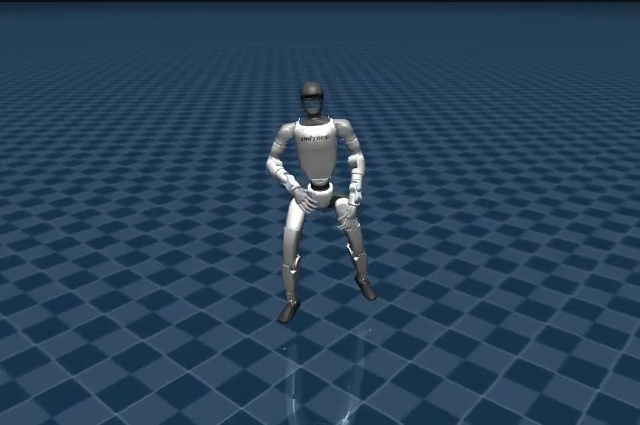
\includegraphics[width=.31\textwidth]{figures/foredance/sequence-10.png} &
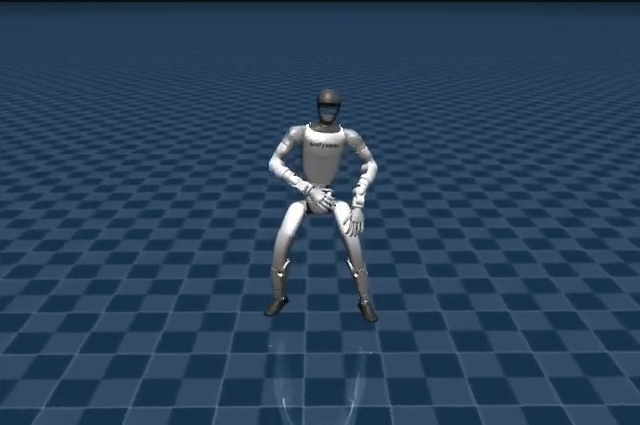
\includegraphics[width=.31\textwidth]{figures/foredance/sequence-30.png} &
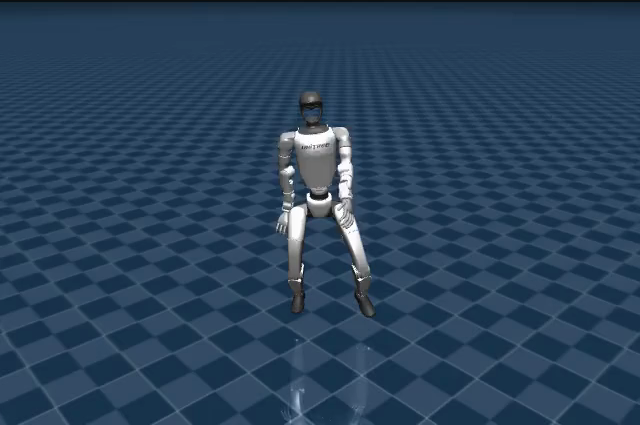
\includegraphics[width=.31\textwidth]{figures/foredance/sequence-50.png}\\
10 seconds & 30 seconds & 50 seconds
\end{tabular}
\par\smallskip
{\small ForeDance: selected 60-second FineDance generation.}

\caption{\textbf{A 60-second ForeDance generation.} Original frames at 10, 30, and 50\,s from a selected FineDance sequence. The images show rendered reference motion.}
\label{fig:sequence}
\end{figure*}

\subsection{Evaluator Validation}
\label{sec:evaluator_validation}
Table~\ref{tab:evaluator_validation} evaluates the score itself on reference
motion. Pairwise accuracy is 68.41\% against ordinary alternative music and
64.08\% against musically similar alternatives. Both exceed random ordering
in point estimate, with the similar-music task providing a more demanding
correspondence check. These results characterize the evaluator's ability to
distinguish soundtracks, rather than the quality of ForeDance generations.

\subsection{Generator Evaluation}
\label{sec:matching_quality}
Table~\ref{tab:mmr_correspondence} reports learned soundtrack correspondence
and beat alignment for generated motion. The intended soundtrack wins
75.01\% of pairwise comparisons, with a mean correct-minus-alternative score
margin of 0.1783. Every generator training seed has a positive mean margin.
The separate 18-track study yields BAS 0.4419. These complementary measures
characterize soundtrack preference and rhythmic alignment; their different
cohorts preclude treating the values as a single pooled evaluation.
Appendix~\ref{app:correspondence_statistics} retains the detailed score
statistics and descriptive intervals.

\paragraph{History-training comparison}
Table~\ref{tab:training} compares clean history, history dropout, and
full-history corruption (FHC), holding the remaining settings fixed.
Relative to clean history, FHC reduces kinetic/geometric FID by
21.9\%/15.0\%, with both directions favorable in all three training seeds,
and increases kinetic diversity. BAS rises from 0.4352 to 0.4419; this is a
descriptive change, not a significance claim. PFC and jerk favor clean
history, so the distribution gains coexist with a smoothness tradeoff.
This comparison examines history regularization, rather than isolating the
benefit of musical anticipation or \cof{}.

\paragraph{Qualitative generation}
\label{sec:showcase}
Figure~\ref{fig:sequence} shows reference poses at 10, 30, and 50\,s from one
selected 60\,s rollout. These original frames illustrate body configuration
across the sequence; they do not measure temporal smoothness.

\subsection{Pending Ablation Studies}
\label{sec:pending_ablations}
\textit{TODO for this working draft: the following controlled studies await
results and are not counted as completed evidence.}

\paragraph{TODO: musical anticipation}
Compare forecast-conditioned and heard-music-conditioned generators with
matched training, tracks, and sampling. Report learned correspondence, BAS,
and motion quality to isolate the value of predictive musical context.

\paragraph{TODO: paired representation training}
Complete current-representation reconstruction and intervention results to
test whether structure and detail serve their intended complementary roles.
Include non-collapse checks and matched supervision comparisons.

\paragraph{TODO: single-representation controls}
Compare independently trained discrete-only, continuous-only, and combined
structure--detail generators under matched settings. Removing a decoder
branch does not substitute for a separately trained baseline.

\paragraph{TODO: committed continuation}
Compare \cof{} with Teacher Forcing on matched 60\,s free-running sequences.
Report aggregate quality and each of the three non-overlapping 20\,s windows,
including commitment-boundary behavior and matched qualitative sequences.

\subsection{Supporting Execution Diagnostics}
\label{sec:execution_results}
The interface in Section~\ref{sec:robot_execution} separates the generated,
resampled, controller-consumed and measured trajectories. The supporting study replays four saved trajectories from one FineDance track
through fixed SONIC in MuJoCo. These trajectories use an earlier 34-dimensional
representation, separate from the current 38-dimensional generation cohort;
audio inference is not run during replay.

After excluding the first two seconds and aligning joint trajectories, median
amplitude retention ranges from 0.858 to 0.901, and median squared-velocity
retention from 0.411 to 0.496. Position tracking therefore coexists with dynamic
attenuation. These diagnostics characterize the reference-to-execution path;
they do not establish current-model hardware performance or comparative
musical benefit. Appendix~\ref{app:execution} retains the complete measurements
and protocol.
